\documentclass[titlepage]{article}
\usepackage[bottom=3cm, right=2cm, left=2cm, top=3cm]{geometry}
\usepackage{graphicx}
\usepackage{hyperref}
\usepackage{float}
\restylefloat{table}
\usepackage{amsmath}
\usepackage{booktabs}

\title{SFWRENG 4NL3 Assignment 2}
\author{Sumanya Gulati}
\date{7 February 2025}

\begin{document}

\begin{titlepage}
    \maketitle
\end{titlepage}

\newpage 

\tableofcontents
\listoftables
\listoffigures

\newpage

\section{Dataset}
% Describe the dataset you chose and why you think it is interesting or useful to analyze.
The dataset I chose consists of transcripts of US Supreme Court Nomination Hearings held by the Congress from 
1971 till 2024. For the scope of this assignment, three women, namely, Justice Sandra Day O'Connor, Justice Ruth 
Bader Ginsburg  and Justics Sonia Sotomayor have been included along with four men - Justice Samuel Alito, Justice 
Anthony Kennedy, Justice John Roberts and Justice Antonin Scalia.\\

In 1981, then US President, Ronald Reagen appointed the first woman to the US Supreme Court. This was a century after 
women in the US fought for their right to practice law as attorneys. To put things into perspective, Ruth Bader Ginsburg, 
despite graduating from Harvard Law School could not find a job as a practicing attorney at any law firm because of gender-based 
discrimination. Through her unwavering determination, she co-founded the Women's Rights Project at the American Civil Liberties 
Union (ACLU).\\

With such blatant discrimination on the basis of sex in the domain of law, I was curious to find whether the society's attitude 
towards women has changed over the past few decades. Using the transcripts from the supreme court nomination hearings, I wish to 
analyze the attitude and mindset of the senators questioning these nominees. The difference in the lenses through which men and 
women with equal qualifications are judged for the same job is pretty obvious. While women are questioned about their committment 
towards their family, how they plan on maintaining a work-life balance, their personality and whether they're amiable; the men
are judged based on their professional qualifications with more focus put on their competency.\\

Through this assignment, I hope to see results that are consistent with this widespread belief and show the inherent bias so many 
people still carry when interviewing equally competent individuals for the same job.

\subsection{Data Collection and Splitting}
% How did you collect the data, choose the categories, and split it into documents?
This dataset has been curated using publicly available data on the \href{https://www.govinfo.gov/collection/supreme-court-nomination-
hearings}{Supreme US Government Information website.}. For each individual in both the categories, the following transcripts from the
hearing have been included - 

For each nomination hearing, the following files have been included as individual documents:
\begin{itemize}
    \item Statements of Committee Members (including Prepared Statements)
    \item Statements and/or Testimony by the Nominee
    \item Questions and Answers
\end{itemize}

These PDFs (each corresponding to one individual document) were manually downloaded and saved in separate 
folders. This data can be found in the \texttt{female-nominees} and \texttt{male-nominees} folders, respectively.

\subsection{Description}
% Include tables and figures to show the size of your dataset, e.g. a table with the number of
% documents and the average number of tokens per document, broken down by category.
The \texttt{text\_extract.py} script was then used to extract all the data from the PDFs and save them as .txt files which can be found
in the \texttt{female-nominees-processed} and \texttt{male-nominees-processed} folders. For the purpose of this assignment, each text file 
in the folders is considered a document. Additionally, two categories - \emph{female nominees} and \emph{male nominees} have been created.
This means that, for the former category, there are 136 documents and for the latter, 147 documents in total. \\

Table \ref{tab:tokens} lists the average number of tokens and the average number of unique tokens per category.

\begin{table}[H] \label{tab:tokens}
    \centering
    \begin{tabular}{lll}
    \toprule
    \textbf{Category} & \textbf{Average Number of Tokens} & \textbf{Average Number of Unique Tokens}\\
    \midrule
    Female Nominees & 4282.378 & 835.897 \\
    Male Nominees & 2024.15 & 593.68 \\
    \bottomrule
    \end{tabular}
    \caption{Average Number of Tokens Per Category}
\end{table}

This is also visualized in figure \ref{fig:tokens} which evidently displays that the number of tokens per document for the female 
nominees is twice as much as that of male nominees. The difference between the average number of unique tokens for the two categories 
is not as sigficant, however.

\begin{figure}[H]\label{fig:tokens}
    \centering
    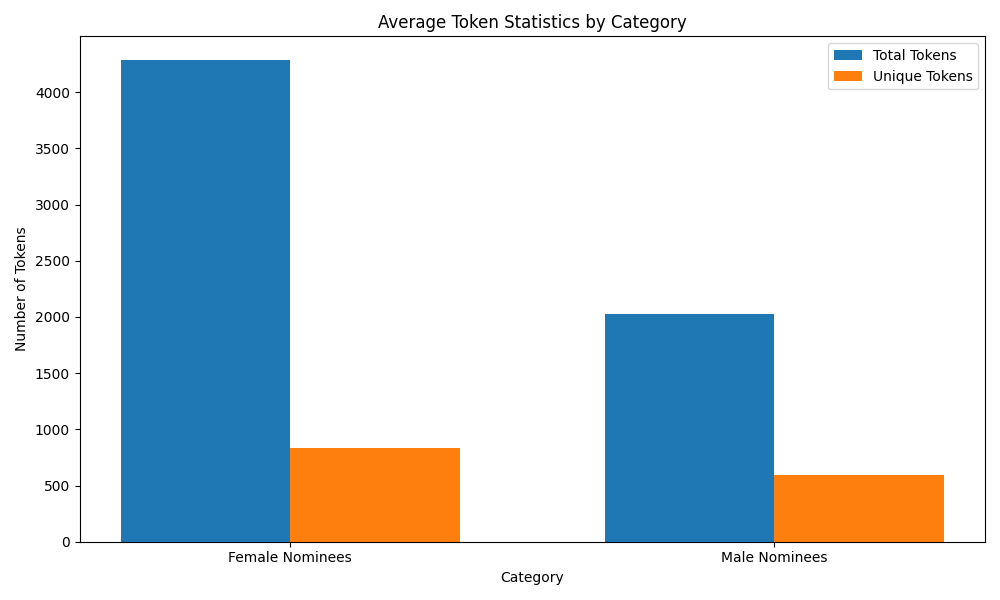
\includegraphics[scale=0.7]{/Users/sg/Desktop/courses/winter-2025/4nl3/assignments/assignment-2/dataset/visualizations/token_statistics.png}
    \caption{Tokens Per Category}
\end{figure}
 
\section{Methodology}
% Describe the steps that you performed and what informed your decisions.
% For example, if you decided not to lowercase the text because it gave better results at a later
% stage, include that decision and your reasoning for doing that. This should include details
% of your preprocessing steps, e.g. lowercasing, stemming, not just saying “each document was
% preprocessed”. Describe the kind of analysis you performed. For any steps that you did not
% implement yourself (e.g. topic modeling), you should mention which package/library was
% used.

\subsection{Preprocessing}
Since the \texttt{data\_extract.py} file only extracts the data from the PDF and store it in a text file, 
the first step in preprocessing the dataset was to clean the text. This was accomplished using the following 
methods through iterative testing:
\begin{itemize}
    \item Replacing all new lines with a blank space.
    \item Removing all words that have a hyphen followed by a blank space. For example, long- term to longterm.
    \item Removing all leading and trailing spaces along with the replacement of multiple blank spaces with a single space.
    \item Removing all digits to streamline the frequency count and ranking of alphabetic tokens. This was implemented 
    because with the digits in the corpus, the years and other random numbers referencing legal cases and such populated the 
    top 10/top 25 counts corrupting the data analysis.
    \item Removing all punctuation for more accurate tokenization.
\end{itemize}

\subsubsection{Naive-Bayes}
Further preprocessing for Naive-Bayes included the following steps:
\begin{itemize}
    \item Using the list of common stopwords from the \textsl{nltk} library to remove words that do not reflect the 
    actual content.
    \item The list of stopwords was expanded to account for commonly found words in the dataset that did not convey the 
    sentiment or the content of the sentence. This includes words such as \texttt{said, would, one, jan, feb}.
    \item To further refine our results, commonly used legal jargon was also added to the list of stopwords. This includes
    words such as \texttt{hearings, committee, senator, judge, case}.
\end{itemize}

\subsubsection{Latent Dirichlet Allocation (LDA) Preprocessing}
Further preprocessing for LDA included the following steps:
\begin{itemize}
    \item Adding additional stop words including `sgpohearings' and `sgpohearingstxt' that are not actual words with defined meanings.
    \item Using NLTK's lemmatizer removing any tokens starting with `sgpo'.
\end{itemize}

\subsection{Bag-of-Words Representation}
As shown in tutorials, the \texttt{CountVectorizer()} function was used to implement Bag-of-Words on the dataset.
Probability calculations given in the instructions PDF for this assignment were then used to implement the 
\texttt{calculate\_word\_probabilities()} function. The output from this function was then to calculate the 
Log Likelihood Ratio. 

\subsection{Naive-Bayes Model}

Given the fact that the dataset is made up of real transcripts of legal hearings, the used of names of the judges and/or
the senators interviewing them are over-represented in the dataset. This skews the results of analyses performed 
on the processed dataset. \\

To combat this issue and to maintain the focus on the goal of this assignment, classifications were establish so the focus of 
the analyses would remain on words that align with the characteristics of the nominee. 4 different classifications - 
Legal Interpretation, Background Experience, Personal Characteristics and Competency Qualification were created. \\

Each of these classifications was populated with a list of related words that speak to that particular classification, such as - 
words like `ruling', `precedent', `principle', `rights' and more were added to the Legal Interpretation classification. By analyzing the 
frequency of these words in the vocabulary for the female and male nominees, any potential bias towards a nominee can be spotted. If 
the focus of the hearing is on 1-2 classifications as opposed to a general overview of all of them, this would highlight implicit bias.

\subsection{Topic Modelling}
The \texttt{gensim} and \texttt{pyLDSvis} libraries were used to implement LDA topic modelling as shown in the tutorial. 
The \texttt{get\_topic\_words()} and \texttt{get\_document\_topic()} functions were then used to get information on the topics and 
documents.  

\subsection{Experimentation}
In addition to importing all the functions from the \texttt{processing.py} file, two new functions were added to implement text normalization 
variation and LDA variation. \texttt{PorterStemmer()} was used to implement stemming as a part of the preprocessing of the data. Another function 
was then implemented to create a TF-IDF matrix using the \texttt{TfidfVectorizer()} function. The code for this was based on the tutorials.

\section{Results and Analysis}
% Present your results as formatted tables and figures. You should
% have at least one table or figure for each of 2.3, 2.4, and 2.5. This must include at least the
% results of the required steps, but may also include any interesting findings you came across
% (e.g. results of topic modeling with and without a given preprocessing step that made a
% difference in the quality of the results). For each table and figure, include a description of
% your main takeaways.
The results and insights gather from the analyses has been summarized in the following subsections.

\subsection{Naive-Bayes}

\begin{table}[H] \label{tab:naive-bayes}
    \centering
    \begin{tabular}{llll}
    \toprule
    \textbf{Gender} & \textbf{Category} & \textbf{Word} & \textbf{LLR Score} \\
    \midrule
    female & background experience & backgrounds & 1.931906639972084 \\
    female & background experience & experienced & 1.0156159080979297 \\
    female & background experience & experiences & 1.9682742841429581 \\
    female & background experience & framework & 2.52789007207838 \\
    female & background experience & services & 1.4982706548972224 \\
    \midrule
    female & personal characteristics & biases & 1.6645918703447364 \\
    female & personal characteristics & ethnicity & 2.6250538205320293 \\
    female & personal characteristics & gender & 1.0750667224516768 \\
    female & personal characteristics & genderbased & 2.10180567676748 \\
    female & personal characteristics & grace & 1.2751271035830118 \\
    female & personal characteristics & identity & 1.1209764237557547 \\
    \midrule
    female & competency qualification & applicability & 1.8941663119892365 \\
    female & competency qualification & availability & 1.46928311802397 \\
    \midrule
    male & legal interpretation & judicially & 1.1407866747180364 \\
    male & legal interpretation & overruling & 1.2014112965344719 \\
    \midrule
    male & background experience & practiced & 1.4245548478486825 \\
    male & background experience & worker & 1.0762481535804653 \\
    male & background experience & workload & 1.4817132616886308 \\
    \midrule
    male & personal characteristics & beliefs & 1.3067718121922978 \\
    male & personal characteristics & embraced & 1.7693953341404107 \\
    male & personal characteristics & unbiased & 2.0570774065921924 \\
    \midrule
    male & competency qualification & disability & 1.209779546204988 \\
    male & competency qualification & wellqualified & 2.0570774065921924 \\
    \bottomrule
    \end{tabular}
    \caption{Results from the Naive-Bayes Analysis}
\end{table}

As shown in table \ref{tab:naive-bayes}, the analysis shows that when interviewing female nominees are interviewed, greater focus 
is put on their personal characteristics with conversations about biases, gender, grace and identity taking up a significant amount 
of attention. In terms of their background experiences and competency qualifictaions, the focus is put on their availability and 
the top words from the category across documents are neutral in tone. None of the words added to the legal interpretation category 
were found in a significant frequency for the female nominees. \\

As for the male nominees, however, words like `judicially' and `overruling' are highlighted showing the focus on the conversation around 
the nominee's career in law and their judgments. The conversations around personal characteristics seem to be more focused on the 
individual as opposed to their gender or other aspects of their identity. The most starking difference can be seen in the tone of 
the competency qualifications since the word `wellqualified' seems to have a very high probability showing the appreciative tone 
of the hearings.

\subsection{Topic Modelling}

The complete list of topic words along with their labels can be found in the \texttt{topic\_words.csv} file. The averages for the top 
20 of these topics split by the gender can also be found in the \texttt{category\_topics.csv} file. 

\begin{figure}[H]\label{fig:LDA}
    \centering
    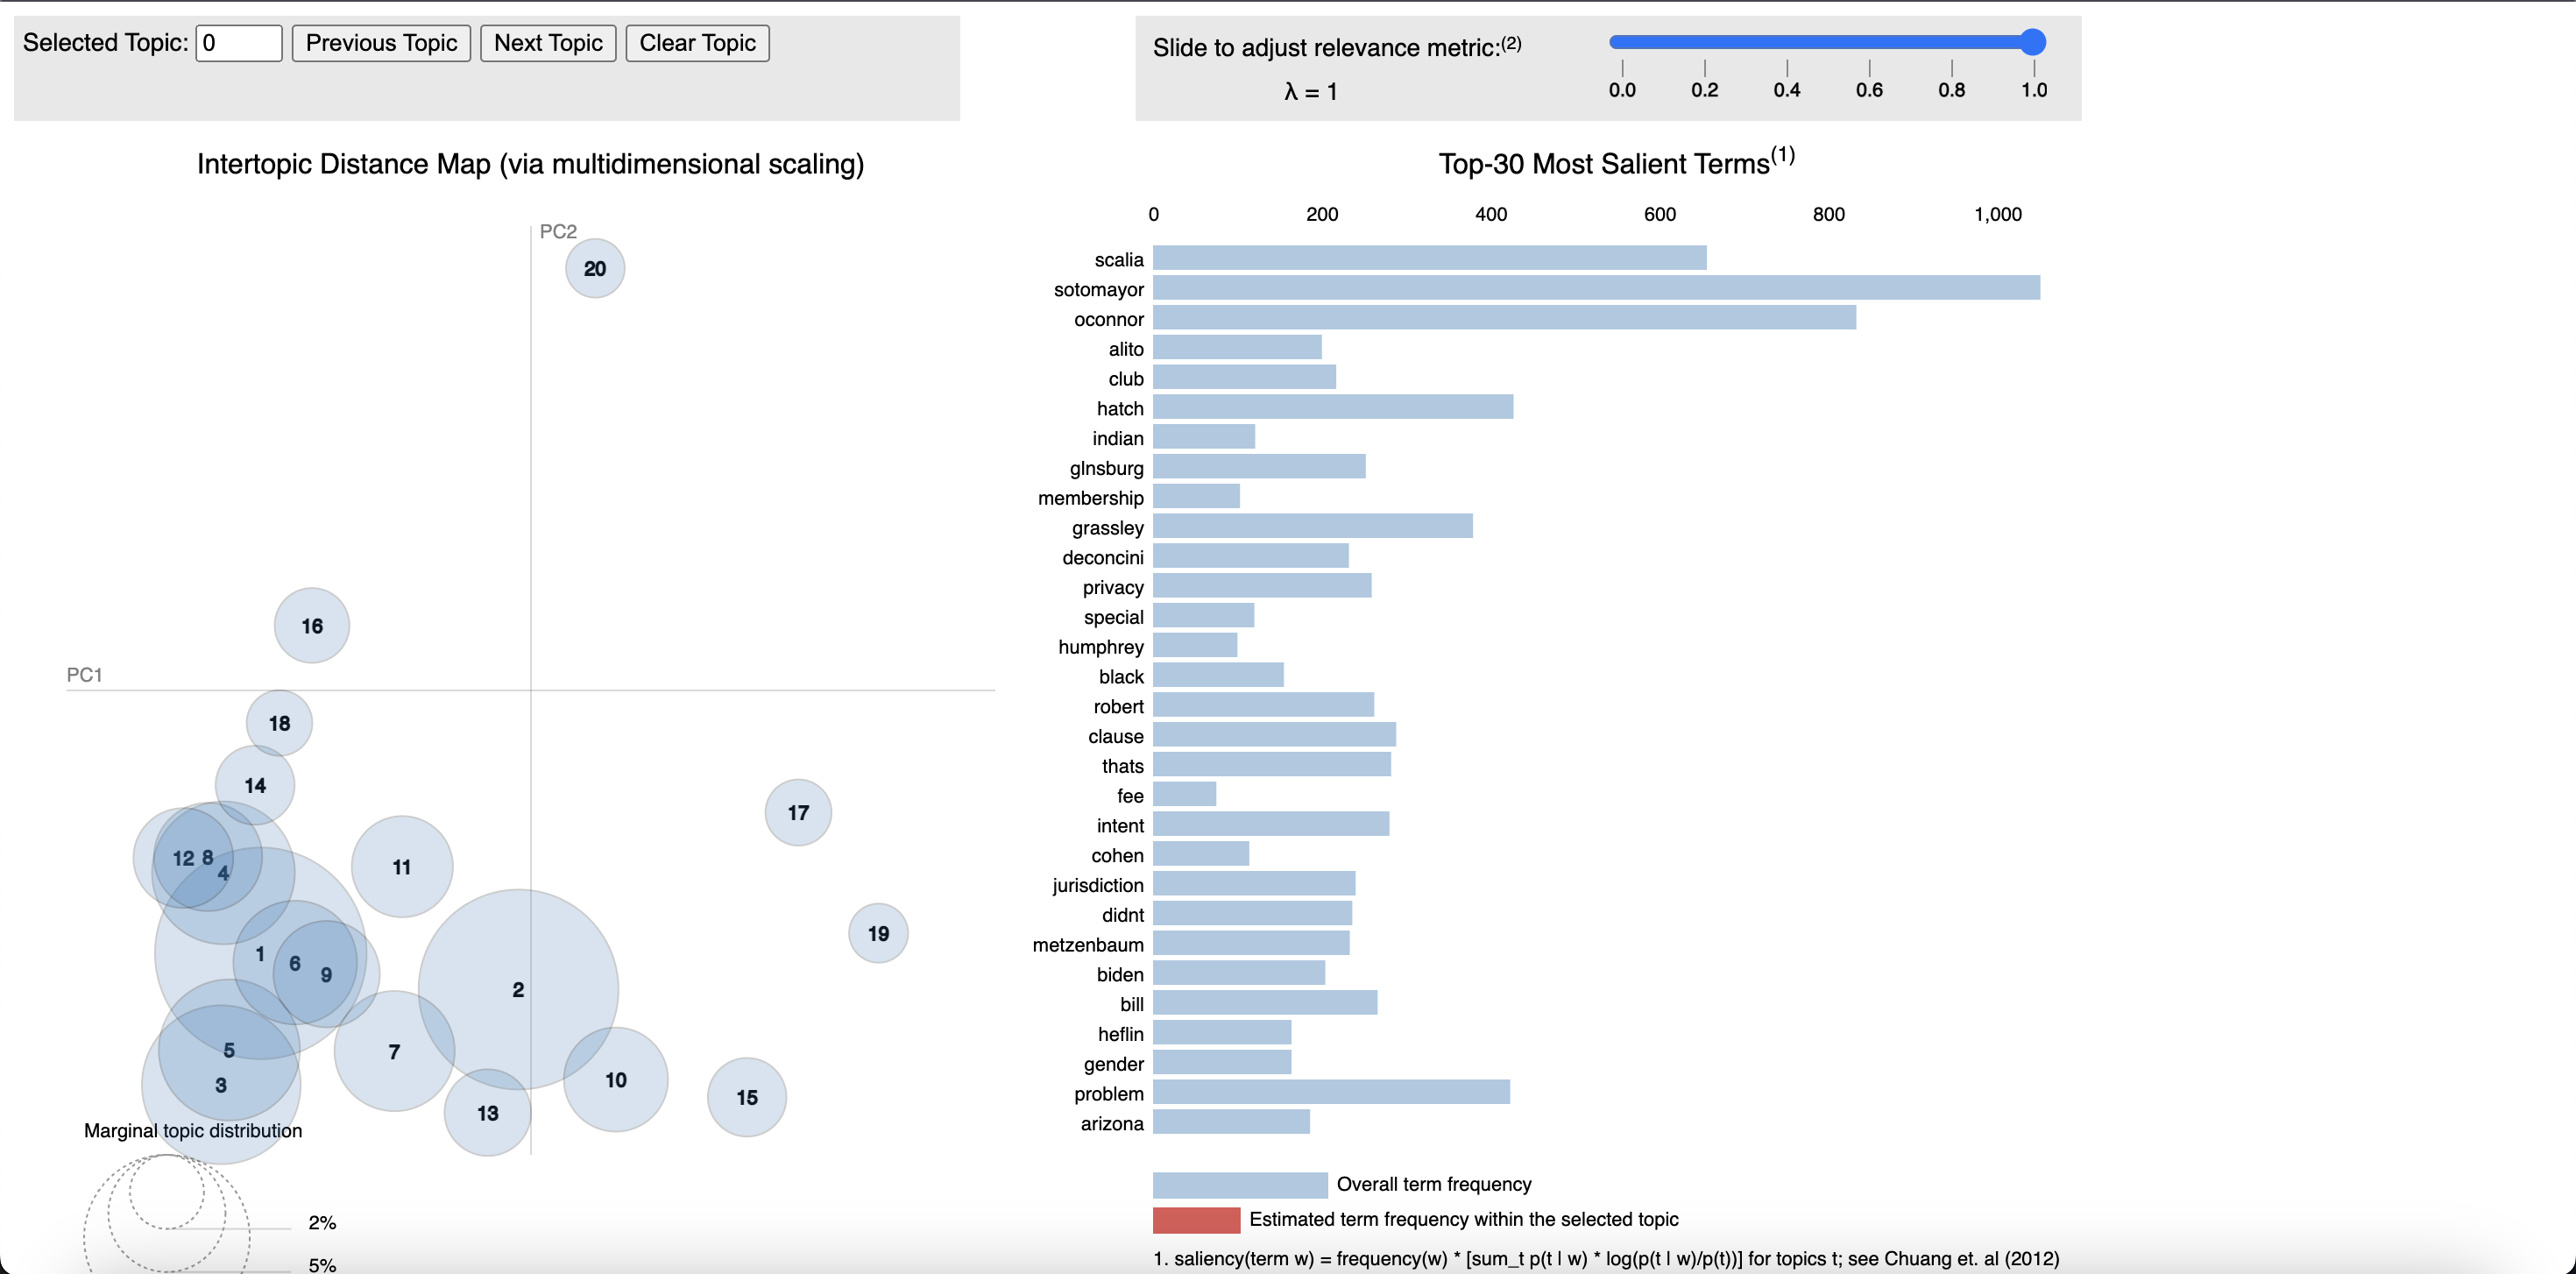
\includegraphics[scale=0.35]{/Users/sg/Desktop/courses/winter-2025/4nl3/assignments/assignment-2/dataset/visualizations/LDA.png}
    \caption{Results from LDA Topic Modelling}
\end{figure}

As shown in figure \ref{fig:LDA}, the intertopic distance map visualizes the relationship between the different topics where each bubble represents 
a topic with the bubble's size indicating the topic's overall prevalence in the dataset. Topics 12, 8, 4, 1, 6, 9, 5, 3 and more are overlapping and 
clustered together suggesting similarity. \\

The 30 most important words are either names, identity-related terms (gender, black) or general legal jargon. 

\subsection{Experimentation}
\begin{figure}[H]\label{fig:stemming}
    \centering
    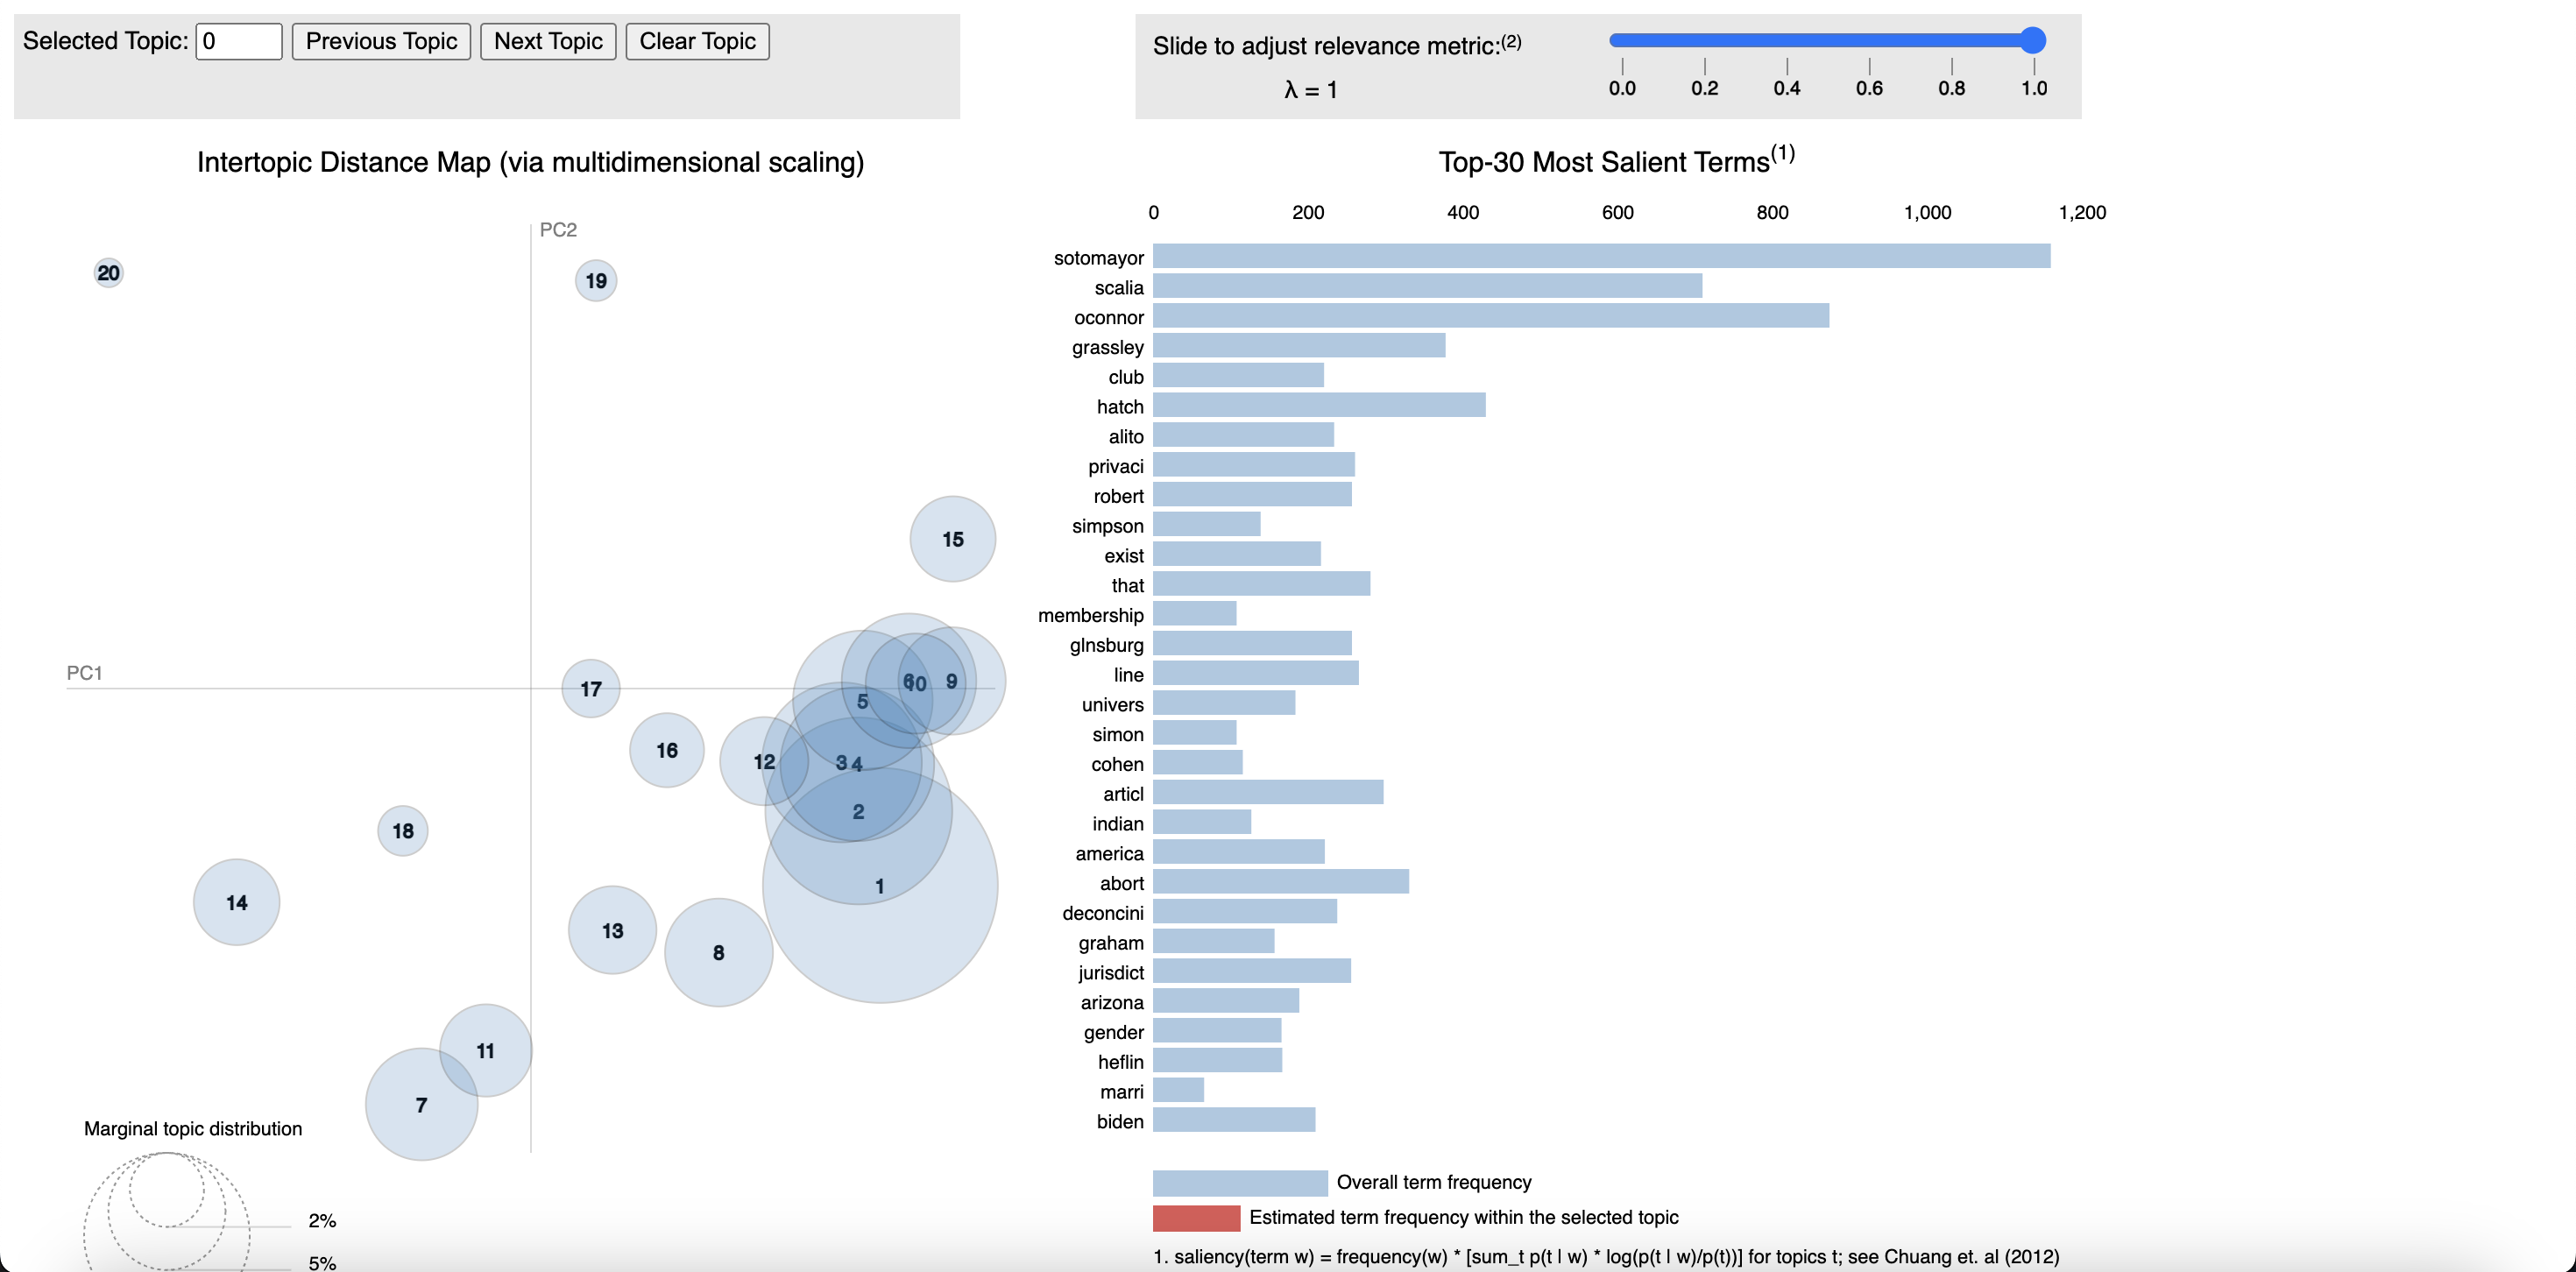
\includegraphics[scale=0.35]{/Users/sg/Desktop/courses/winter-2025/4nl3/assignments/assignment-2/dataset/visualizations/stemming_LDA.png}
    \caption{Results from LDA Topic Modelling Post-Stemming and with TF-DIF}
\end{figure}

As shown in figure \ref{fig:stemming}, the intertopic distance map visualizes the relationship between the different topics where each bubble represents 
a topic with the bubble's size indicating the topic's overall prevalence in the dataset. Topics 5, 6, 10, 9, 3, 4, 2, 1 and more are overlapping and 
clustered together suggesting similarity. \\

The list of the 30 most popular words seems to have a lot of incomplete words suggesting improper text preprocessing and analysis.

\section{Discussion}

\subsection{Findings}
% Include two subsections in the discussion. The first should talk about what
% you learned about your dataset. Imagine that you are describing what your results showed,
% at a high level, to a friend who does not have any NLP experience but is interested in the
% corpus that you chose.

\subsection{Reflection}
% The second subsection should cover what lessons you personally
% learned during the completion of the assignment. You might write about how you found and
% processed the data, preprocessing effects on downstream analysis, topic modeling results,
% limitations of your approaches, or other interesting aspects that were new to you.

\section{Appendix}

\end{document}